\chapter{Approach}
\label{chap:approach}
There are four steps in the design and implementation of the portable probabilistic programming framework. At first we designed the syntax of the embedded programming language, which targets the description of the Bayesian networks and conditional query.  The design of the language is based on BUGS, but the syntax is more specific and efficient to be lightweight for the portable characteristic. Also the syntax can be expressive for most of the probabilistic models. The description of the models using the portable probabilistic programming language is separated from the code of the host language as well of the conditional query, which can enhance the reusability of the probabilistic models. The parser is implemented and the inference engine is generated automatically based on the conditional query. More details will be illustrated in section ~\ref{sec:syntax}. 

We implemented the probabilistic library for most of the probabilistic distribution such as Gaussian, Gama, Beta, etc. Our probabilistic programs define distributions by defining a distribution over possible execution traces. The distribution is fully specified by a generative procedure. More details can be found in section ~\ref{sec:distr}. 

The inference algorithm is based on the MCMC sampling, such as Gibbs Sampling or Metropolis-Hastings Algorithm, which is efficient and lightweight to implement. We will elaborate more on the mechanism of the inference engine through an example in section ~\ref{sec:infer}. 

Additionally, we implement the APIs for other languages leveraging some existing development tool such as SWIG (Simplified Wrapper and Interface Generator). More details for the APIs are in section ~\ref{sec:api}.

Our main contribution lies in the design of the portable probabilistic programming language to make it portable, the implementation of the probabilistic library and the lightweight implementation of the inference engine.


\section{Syntax of programming language}
\label{sec:syntax}

An example describing the flip model in our language is showed in Figure ~\ref{fig:flip_eg}. 

\begin{figure}
    \centering
    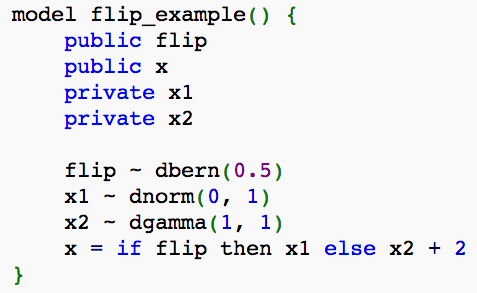
\includegraphics[width=0.6\textwidth]{figures/flip_eg.png}
    \caption{Flip example, describing the probabilistic model in our language.}
    \label{fig:flip_eg}
\end{figure}

The flip\_example describes a probabilistic model that has the distribution over variables as showed in Figure ~\ref{fig:flip_dist}. Part of the syntax in this example is showed in Figure ~\ref{fig:flip_syn}. Under this syntax, the parser will parse the probabilistic program and generate the Bayesian network as the user described. The inference is done based on the probabilistic graph. The Bayesian network of the flip example is showed in Figure ~\ref{fig:flip_net}.


\begin{figure}
    \centering
    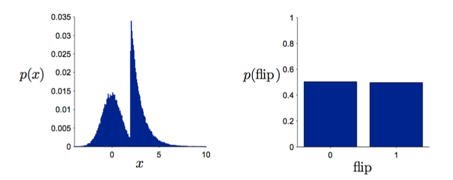
\includegraphics[width=0.9\textwidth]{figures/flip_dist.png}
    \caption{Flip example, the implied distributions over variables.}
    \label{fig:flip_dist}
\end{figure}

\begin{figure}
    \centering
    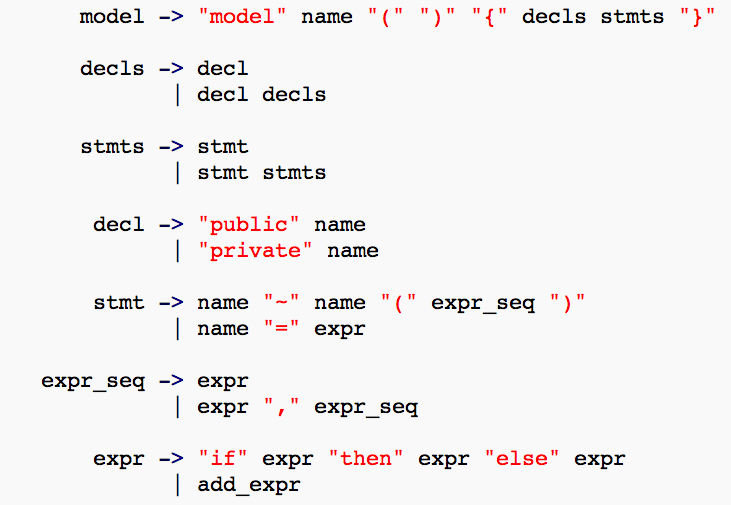
\includegraphics[width=0.7\textwidth]{figures/flip_syn.png}
    \caption{Part of the syntax of the language in flip example.}
    \label{fig:flip_syn}
\end{figure}


\begin{figure}
    \centering
    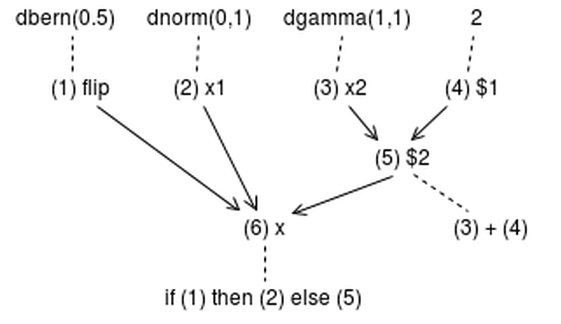
\includegraphics[width=0.6\textwidth]{figures/flip_net.png}
    \caption{The generated Bayesian network for the flip example.}
    \label{fig:flip_net}
\end{figure}


\section{Probabilistic distribution library}
\label{sec:distr}
We implemented the probabilistic library for most of the probabilistic distribution such as Gaussian, Gama, Beta, etc. Our probabilistic programs define distributions by defining a distribution over possible execution traces. The distribution is fully specified by a generative procedure. Some complex distributions are crafted compositionally. An example is showed on how to implement a Gaussian Mixture Model distribution in Figure ~\ref{fig:gmm}. As can be seen in Figure ~\ref{fig:gmm}., everytime we run the function gmm(), it will return a value based on the distribution implementation. And the trace of the returned value will meet the requirements of the density probability the program has defined.


\begin{figure}
    \centering
    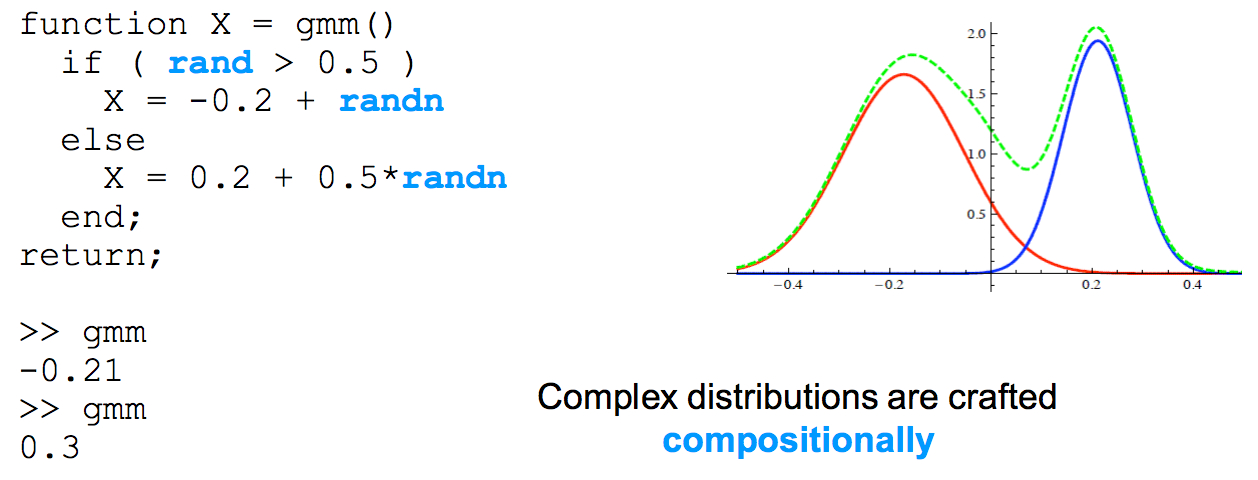
\includegraphics[width=0.9\textwidth]{figures/gmm.png}
    \caption{Implementation of GMM distribution example.}
    \label{fig:gmm}
\end{figure}


Most of the distributions in our library are implemented based on Normal distribution and Bernoulli distribution according to the mathematical methods. The probabilistic distributions in our library contain Bernoulli distribution, Normal distribution, Gamma distribution, Binomial distribution, Multinomial distribution, Dirichlet distribution, Beta distribution, Uniform distribution, and Poisson distribution.

\section{Inference engine}
\label{sec:infer}
Probabilistic inference is the problem of computing an explicit representation of the probability distribution implicitly specified by a probabilistic program. If the probability distribution is over a large number of variables, an explicit representation of the joint probability distribution may be both difficult to obtain efficiently, and unnecessary in the context of specific application contexts. For example, we may want to compute the expected value of some function f with respect to the distribution (which may be more efficient to calculate without representing the entire joint distribution). Alternatively, we may want to calculate the most likely value of the variables, which is the mode of the distribution. Or we may want to simply draw a set of samples from the distribution, to test some other system which expects inputs to follow the modeled distribution.
Figure ~\ref{fig:infer_eg}. gives an example of inference problem.

\begin{figure}
    \centering
    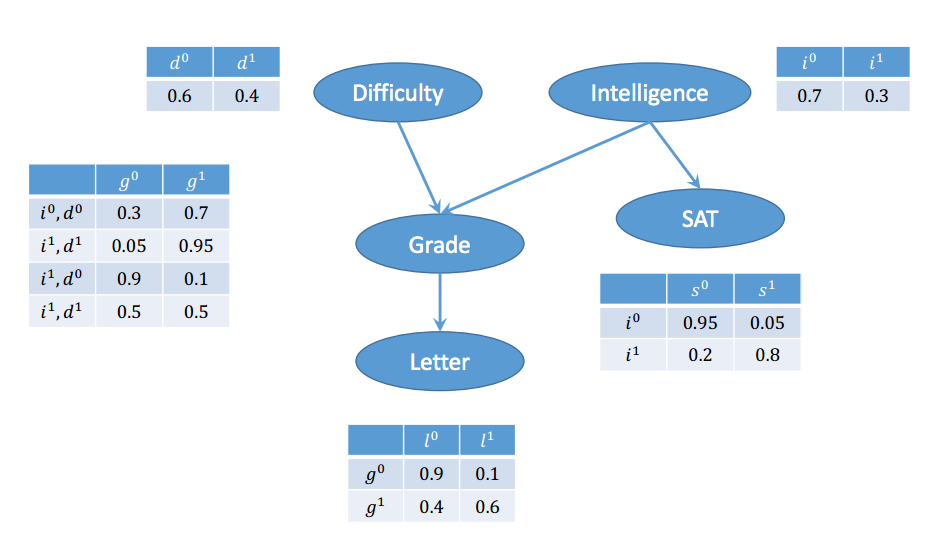
\includegraphics[width=0.9\textwidth]{figures/inference.png}
    \caption{A student example to show probabilistic inference.}
    \label{fig:infer_eg}
\end{figure}


As is showed in Figure ~\ref{fig:infer_eg}., the variable Difficulty describes the difficulty of the courses with probability 0.6 to be not hard, namely d0, and probability 0.4 to be d1. Other variables share the similar meaning with Difficulty. If we want to know the probability of the student can get Letter = l1 under the condition his grade Grade = g1, then this is an inference problem with the formal representation P (L = l1 | G = g1). Also, if we want to know the probability of the student getting Grade = g1 under he/she has already get the Letter = l1, which is backward compared with the previous conditional probability, this is also the problem of probabilistic inference with the formal representation P (G = g1 | L = l1).

The mechanism of the inference engine is based on sampling. Currently we use Rejection Sampling algorithm in the inference engine, which is straightforward and easy to implement. The intuitive idea is to sample the traces as the program runs. If the trace meets the Boolean requirements of the condition, then record the trace, or the trace is discarded. Then we calculate the number of the traces that can meet the Boolean requirement of the probability we want to get. Then calculating this number over the whole number of traces we recorded can derive the final conditional probability. 

Sampling methods all approximately get the probability, but compared with exact inference the former can be more efficient. Rejection Sampling is straightforward and it is not as efficient as other sampling algorithms. There are other suitable sampling algorithms like Gibbs Sampling and Metropolis-Hastings algorithm that we have investigated and we will add these algorithms to our inference engine in the future.

\section{APIs for other languages}
\label{sec:api}
We leverage the development tool SWIG (Simplified Wrapper and Interface Generator) ~\cite{swig} to make other languages be able to call for C functions, as we implemented in C. Once the user has the APIs, he/she is able to call the load probabilistic model function or inference function in each common language. That how the portable is implemented. 

	The only challenge in this part is the C/C++ pointer doesn’t exist in other languages like Java and Python. We cope with this problem by using wrapper with a specific form to hint the difference of the pointers and the normal variables.
